\chapter{Projekt systemu}
\label{chap:ProjektSystemu}

Brak dostępnego na rynku systemu wspierającego monitorowanie klienta
mobilnego powoduje konieczność opracowania nowego rozwiązania, które
spełni wszystkie wymagania opisane w~\ref{chap:Wymagania}. Opracowanie
od podstaw nowego systemu monitorowania, wymaga bardzo dużych nakładów
pracy. Na rynku obecne są systemy monitorowania klienta statycznego,
które spełniają znaczną część wymagań. Implementacja nowego systemu
monitorowania jest zatem nieuzasadniona ekonomicznie oraz
merytorycznie. Na podstawie wyników analizy dostępnych na rynku
systemów podjęto decyzję, aby wykorzystać system monitorowania Icinga.

Zastosowanie systemu Icinga pozwala na uzyskanie niskim nakładem
pracy, wielu funkcjonalności niezbędnych w~projektowanym
systemie. System monitorowania Icinga jest jednym
z~najpopularniejszych narzędzi służących do monitorowania
infrastruktury statycznej. Posiada on bardzo wiele konfiguracji
rozproszonych, zatem możliwe jest monitorowanie nawet bardzo
rozbudowanej sieci. Wiele dostępnych dodatków pozwoli również na
zapewnienie możliwości analizy danych zarówno historycznych jak
i~bieżących. Łatwo zatem zauważyć, że dzięki zastosowaniu systemu
dostępnego na rynku uzyskano realizację znacznej części
wymagań. System nie posada jednak żadnych zintegrowanych mechanizmów
monitorowania klienta mobilnego. Konieczne jest zatem opracowanie
dodatkowych elementów, które pozwolą na monitorowanie klienta
mobilnego zgodnie z~przedstawionymi wymaganiami.

Klient mobilny, zdefiniowany w~\ref{chap:Wymagania} jest urządzeniem,
co do którego, nie można zakładać, że posiada nieprzerwany dostęp do
sieci internet. Ponadto należy zauważyć zmienność zarówno
geograficznego miejsca użytkowania jak i~topologi wykorzystywanej
infrastruktury sieciowej. Dodatkowo, należy odnieść się do wymagań,
w~których zawarta jest konieczność minimalizowania zużycia energii
przez klienta mobilnego. Ciągłe utrzymywanie połączenia z serwerem,
powodowałoby znaczne zużycie energii. Współpraca klienta mobilnego
z~infrastrukturą publiczną nie pozwala również, na założenie, iż
klient mobilny posiada globalny adres IP\footnote{Globalny adres IP -
  adres protokołu internetowego działającego w warstwie sieciowej,
  pozwalający na unikalną identyfikację urządzenia w ramach całej
  sieci Internet.}. Wszystko to razem powoduje to brak możliwości
wykorzystania mechanizmów aktywnego monitorowania zawartych w~systemie
Icinga do monitorowania klienta mobilnego.

Brak możliwości inicjowania przez system monitorujący komunikacji
wymusza użycie jednej z~dwóch dostępnych konfiguracji
rozproszonych. Pierwsza konfiguracja, zakłada przekazywanie jedynie
rezultatów pomiarów do jednej z~instancji rdzenia monitorującego,
który następnie dokona ich przetwarzania. Po wykonaniu wszystkich
niezbędnych czynności rezultaty zostaną dostarczone do centralnej bazy
danych. Druga z~konfiguracji, zakłada wykonanie całej niezbędnej
analizy danych na urządzeniu mobilnym, a~następnie przekazanie
rezultatów do bazy danych. Charakterystyka klienta mobilnego
przedstawiona w~\ref{chap:Wymagania}, określa iż urządzenie mobilne
posiada ograniczone zasoby i~ilość dodatkowych operacji wykonywanych
na nim powinna zostać ograniczona do minimum. Powyższe wymaganie
dyskwalifikuje rozwiązanie, które wymaga przetwarzania wyników
pomiarów na urządzeniu mobilnym. Konieczne jest zatem wykorzystanie
konfiguracji, w~której na urządzeniu mobilnym znajduje się narzędzie
przeznaczone jedynie do zbierania danych oraz przekazywania ich do
nadrzędnej instancji jądra monitorującego. W~klasycznym wariancie tej
konfiguracji, która wykorzystywana jest podczas monitorowania
infrastruktury statycznej, do przekazywania danych wykorzystuje się
dodatek NSCA. Przeprowadzona w~\ref{sec:NSCA} analiza narzędzia NSCA
oraz protokołu komunikacyjnego wykazała liczne uchybienia tego
narzędzia oraz wykorzystywanego w nim protokołu. Konieczne jest zatem
opracowanie metody komunikacji spełniającej przedstawione wymagania
wcześniej wymagania. Ponadto wiele ograniczeń narzędzia NSCA
spowodowało konieczność zaprojektowania i~implementacji nowego
narzędzia, które jest wolne od ograniczeń poprzednika. Powyższe
czynniki determinują w~znacznym stopniu architekturę system. W~celu
zapewnienia elastyczności projektowanego systemu zastosowano budowę
modularną. Schemat współpracy poszczególnych modułów został
przedstawiony na \ref{fig:archCalosci}. System monitorowania składa się
z~następujących modułów:

\begin{figure}[ht]
  \caption{Schemat logiczny projektowanego systemu.}
  \label{fig:archCalosci}
  \centering
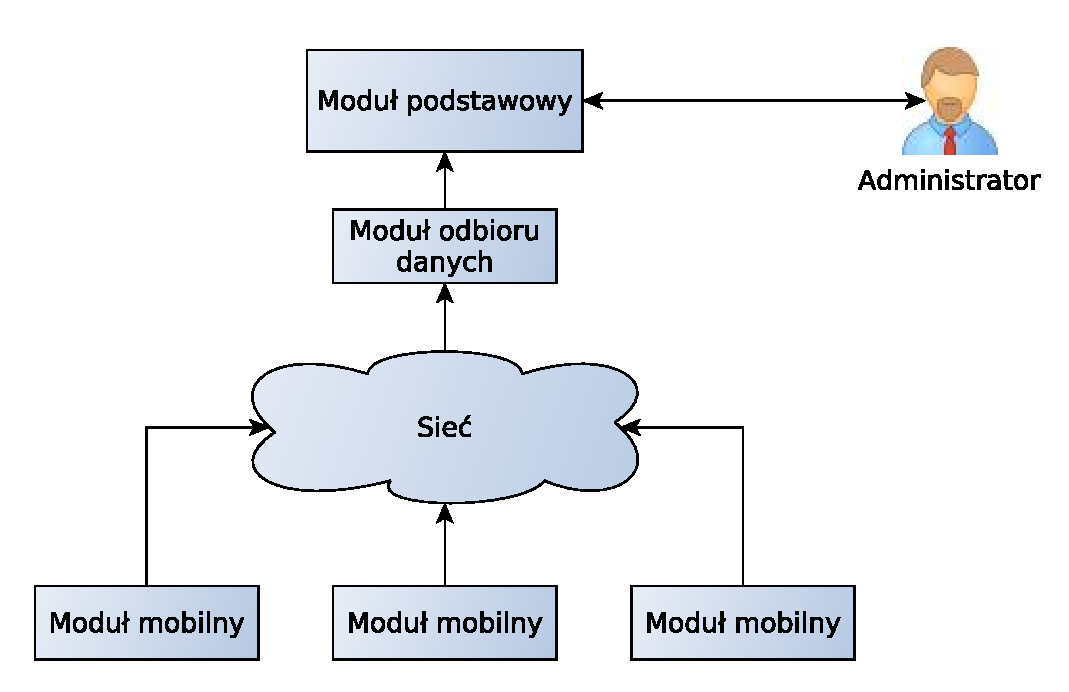
\includegraphics[width=0.8\textwidth]{img/archCalosci}
\end{figure}

\begin{description}
\item[Moduł podstawowy] Zawiera wszystkie instancje rdzenia
  monitorującego, zarówno te wykorzystywane do monitorowania
  infrastruktury statycznej, jak i~te których zadaniem jest
  przetwarzanie danych pochodzących od klientów mobilnych. Ponadto
  w~module tym zawiera się interfejs użytkownika wraz ze~wszystkimi
  dodatkami oraz magazyn danych.

\item[Moduł odbioru danych] Składa się on z~programu, który zapewnia
  odbiór danych od klienta mobilnego przy zachowaniu wszystkich
  wymagań zarówno w~kwestii bezpieczeństwa jak
  i~funkcjonalności. Ponadto moduł ten odpowiedzialny jest za
  przekazywanie odebranych danych do pozostałych elementów zgodnie
  ze~zdefiniowaną w~systemie polityka.

\item[Moduł mobilny] Zależna od platformy aplikacja mobilna, której
  podstawowym zadaniem jest gromadzenie danych o~zadanych
  parametrach. Zawiera się tu również implementacja protokołu
  komunikacyjnego dla danej platformy w~celu przekazania zebranych
  danych do pozostałych modułów systemu.
\end{description}

\section[Projekt modułu podstawowego][Projekt modułu podstawowego]{Projekt modułu podstawowego}

Moduł ten składa się z~kilku współpracujących ze sobą
elementów. Możliwa jest konfiguracja tego modułu w~kilku wariantach,
co umożliwia dostosowanie go do rozmiarów oraz topologi monitorowanej
infrastruktury. Każda z~stosowanych konfiguracji musi zapewniać
co najmniej poniższą funkcjonalność:

\begin{itemize}
\item monitorowanie infrastruktury statycznej,
\item przetwarzanie danych pochodzących od klienta mobilnego,
\item gromadzenie danych,
\item zapewnienie interfejsu dla administratora.
\end{itemize}

Minimalna konfiguracja modułu musi się składać co najmniej z~jednej
instancji rdzenia monitorującego oraz dowolnego z~interfejsów,
klasycznego lub icinga-web. W~celu umożliwienia przetwarzania danych
pochodzących od klientów mobilnych konieczne jest jedynie
zdefiniowanie tych urządzeń oraz ich usług, jako monitorowane
pasywnie. Należy jednak zwrócić uwagę na liczne ograniczenia tej
konfiguracji, które zostały omówione w~\ref{chap:Icinga}. Ponadto
konfiguracja ta nie spełnia wszystkich wymagań, gdyż nie umożliwia
analizy zgromadzonych danych historycznych. W~celu spełnienia
wszystkich wymagań należy zatem wzbogacić omawianą konfigurację
o~dodatek inGraph, który umożliwi administratorowi analizę
zgromadzonych danych.

Liczne wady przedstawionej konfiguracji powodują, że jej
funkcjonalność jest znacząco ograniczona. Wykorzystanie jej możliwe
jest jedynie w~bardzo małych sieciach, które nie będą już
rozwijane. Zalecana jest zatem konfiguracja o~nieco rozszerzonej
strukturze. W~skład tej konfiguracji wchodzą:

\begin{itemize}
\item rdzeń lub rdzenie monitorujące z~komponentem IDOUtils
\item baza danych systemu Icinga
\item dodatek inGraph
\item baza danych dodatku inGraph
\item interfejs icinga-web
\end{itemize}

\begin{figure}[ht]
\centering
  \caption{Schemat zalecanej konfiguracji systemu.}
  \label{fig:modulPodstawowy}
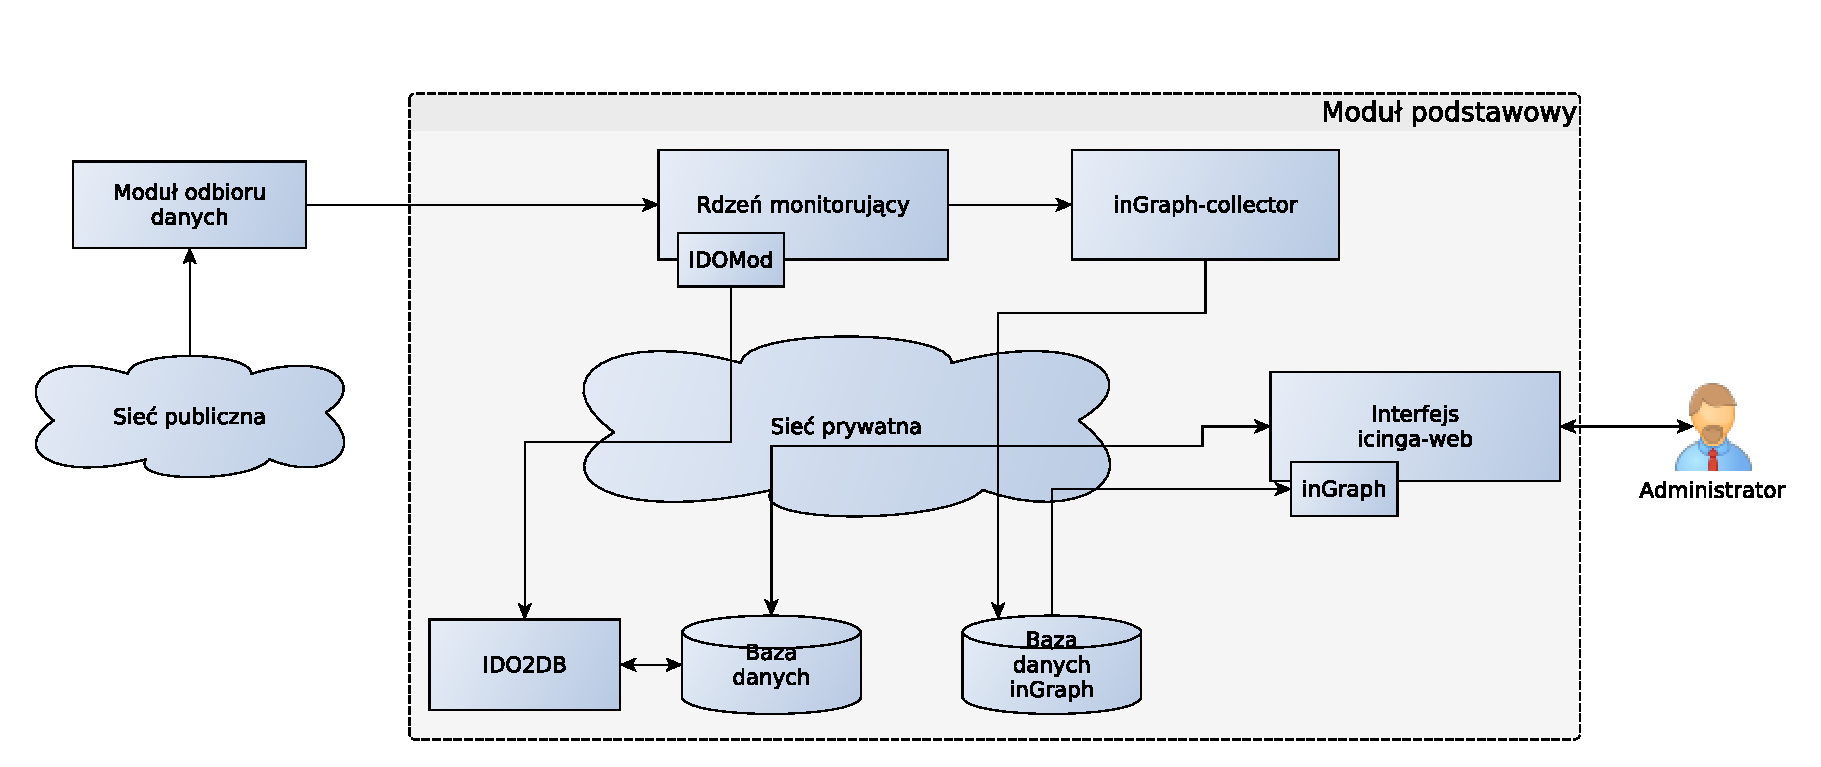
\includegraphics[width=1\textwidth]{img/modulPodstawowy}
\end{figure}

Minimum wymaganym do funkcjonowania tej konfiguracji jest jedna
instancja rdzenia monitorującego. Będzie ona monitorowała zarówno
infrastrukturę statyczną jak i~przetwarzała dane od klienta
mobilnego. Wszystkie dane przetworzone przez tą instancję trafiają do
bazy danych z~której korzysta interfejs użytkownika icinga-web. Taka
konfiguracja umożliwia bardzo dobrą skalowalność całego systemu oraz
łatwego dostosowania go do struktury monitorowanej sieci. Rozbudowa
infrastruktury monitorującej może zostać wykonana w~łatwy sposób
poprzez dodanie kolejnej instancji jądra wykorzystującej tą samą bazę
danych. Ponadto możliwe jest również łączenie tej konfiguracji
z~niemalże dowolną inną konfiguracją bez zaburzania pracy
systemu. Skalowalność tej konfiguracji dotyczy również klienta
mobilnego. Jeśli klientów mobilnych jest zbyt dużo, aby mogły zostać
obsłużone przez jedną instancję, możliwe jest dodanie kolejnej
instancji, która będzie odpowiedzialna za przetwarzanie danych od
wyznaczonej części klientów mobilnych. W~celu umożliwienia analizy
danych historycznych zalecane jest użycie dodatku inGraph. Został on
opisany szczegółowo w~\ref{sec:inGraph}. Jego wykorzystanie umożliwia
prezentację administratorowi zarówno uśrednionych wartości z~długiego
okresu czasu jak i~szczegółowych danych z~zadanego przedziału. W~celu
wykorzystania tego dodatku w~omawianej konfiguracji konieczne jest
umieszczenie elementu zbierającego dane przy każdej instancji rdzenia
monitorującego. Wszystkie zebrane dane zapisywane są w~jednej bazie
danych z~której korzysta interfejs użytkownika.



\section[Protokół komunikacyjny][Protokół komunikacyjny]{Protokół komunikacyjny}
\label{sec:ProtKom}

Wymagania przedstawione w~\ref{chap:Wymagania} definiują bardzo wiele
cech systemu, które muszą być zapewnione poprzez użycie odpowiedniego
protokołu komunikacyjnego. Analiza wymagań pozwoliła na wyodrębnienie
następujących cech protokołu komunikacyjnego:

\begin{description}
\item[spójność danych] protokół musi gwarantować, że dane zostały
  dostarczone i~przetworzone;
\item[integralność] protokół musi zapewniać, że dane zostaną
  dostarczone w~niezmodyfikowanej postaci i~jedynie od
  uwierzytelnionego nadawcy;
\item[poufność] protokół musi zapewniać przekazanie danych w sposób,
  który uniemożliwi stroną trzecim ich odczytanie;
\item[niezależność algorytmu szyfrowania] protokół musi być niezależny
  od algorytmu, którym szyfrowane są dane;
\item[uwierzytelnienie klienta] protokół musi zapewniać element
  pozwalający na potwierdzenie tożsamości klienta;
\item[niezależność uwierzytelnienia klienta] protokół musi być
  niezależny od wykorzystywanej metody uwierzytelnienia klienta;
\item[uwierzytelnienie serwera] protokół musi zapewniać potwierdzenie
  tożsamość serwera;
\item[odporność na utratę urządzenia klienckiego] protokół nie może
  wymagać przechowywania na urządzeniu danych pozwalających na
  kompromitację całego systemu;
\item[oszczędność pasma] protokół powinien minimalizować ilość
  przesyłanych danych.
\end{description}

Rozbudowane wymagania bezpieczeństwa protokołu wynikają
z~charakterystyki przesyłanych danych. Dane, które pochodzą
z~urządzenia mogą zawierać zarówno poufne dane właściciela jak
i~tajemnice handlowe firmy. Ujawnienie tych danych może pociągać za
sobą poważne konsekwencje finansowe lub prawne, dlatego konieczne jest
zapewnienie bezpiecznego protokołu. Należy również pamiętać, że jedna
ze stron komunikujących się przy użyciu protokołu znajduje się na
urządzeniu mobilnym przez co należy ograniczyć narzut wprowadzany
przez użycie tego protokołu.

Spośród bezpiecznych protokołów komunikacyjnych rozpowszechnionych na
rynku najbliższym spełnienia wszystkich wymagań jest protokół Secure
Socket Layer - SSL\footnote{Szczegółowy opis protokołu można znaleźć
  w~\cite[148-155]{book:kryptografia}.}. Jest to protokół warstwy
prezentacji, który pozwala na bezpieczny transport strumienia
danych. Protokół wykorzystuje zarówno kryptografię symetryczną jak
i~asymetryczną. Kryptografia asymetryczna wykorzystywana jest do
uwierzytelnienia serwera i~opcjonalnie klienta przy pomocy
certyfikatów nadawanych przez centra certyfikacji. Model
bezpieczeństwa zastosowany w~tym protokole pozwala przy pomocy kluczy
centrów autoryzacji dokonywać weryfikacji certyfikatów przesyłanych
przez wiele witryn. Niestety głębsza analiza protokołu wykazała, iż
nie spełnia on wszystkich wymagań. Przede wszystkim zestawienie
połączenia wymaga przesłania znaczącej ilości danych. Ponadto
konieczne jest zdobycie certyfikatu, który pozwalałby na weryfikację
serwera. Model bezpieczeństwa zastosowany w~SSL jest dla
rozpatrywanego przypadku nadmiarowy, ponieważ klient mobilny
przekazuje dane zawsze do tego samego serwera. Protokół SSL
przeznaczony jest głównie dla sklepów internetowych oraz banków, gdyż
jest on nastawiony na uwierzytelnienie serwera i~zapewnia bezpieczny
kontakt w wieloma domenami przy użyciu niewielkiej liczby centrów
certyfikujących.

Nadmiarowość modelu bezpieczeństwa protokołu SSL powoduje nadmierne
zużycie pasma. Ponadto zamknięty zbiór algorytmów możliwych
szyfrowania możliwych do wykorzystania powoduje, że nie może on być
zastosowany w~omawianym przypadku. Wobec braku gotowego protokołu
konieczne jest zaprojektowanie nowego, który spełni wszystkie stawiane
wymagania.

Protokół został oparty na protokole TCP, który zapewnia abstrakcję
przesłania strumienia bajtów z~gwarancją ich dostarczenia. Mnogość
wymagań dotyczących projektowanego protokołu utrudnia wykorzystanie
architektury jednowarstwowej. Konieczne jest zatem wydzielenie warstw
z~których każda będzie zapewniała dobrze zdefiniowane usługi dla
warstw wyższych.
 

\subsection[Warstwa formowania wiadomości][Warstwa formowania wiadomości]{Warstwa formowania wiadomości}

Najniższa warstwa protokołu komunikacyjnego zbudowana jest
bezpośrednio na protokole TCP. Komunikujące się strony w swej
architekturze wykorzystują paradygmat programowania
zdarzeniowego. Abstrakcja strumienia bajtów zapewniana przez protokół
TCP nie jest odpowiednia dla tego modelu. Konieczne jest zatem
dostarczenie warstwy, która umożliwi przesłanie w całości komunikatu
o~zadanej długości. Umożliwia to wygodne przesyłanie wiadomości
odpowiadających poszczególnym zdarzeniom w~komunikujących się
programach.

Usługa zapewniana przez tą warstwę jest bardzo prosta, dzięki czemu
rozpoczęcie komunikacji nie wymaga żadnej inicjalizacji. Protokół jest
w~pełni symetryczny. Oznacza to, że obie komunikujące się strony
posiadają taki sam dozwolony zbiór stanów protokołu. Warstwa świadczy
usługę przekazywania wiadomości o~zdefiniowanym rozmiarze. W~celu
wykonania tej usługi, do danych, które są dostarczone stronie
nadawczej dołączana jest ich długość. Długość w~protokole jest
reprezentowana jako 32 bitowa liczba ze znakiem o~sieciowej kolejności
bajtów. Tak sformatowana wiadomość przesyłana jest przy użyciu
protokołu TCP do odbiorcy. Odbiorca po odebraniu pierwszych czterech
bajtów wiadomości sprawdza rozmiar danych, po czym rozpoczyna
odbieranie ilości danych określonej przez nagłówek. Wiadomość jest
przekazywana użytkownikowi dopiero w~momencie odebrania całego
komunikatu. Jeśli w~trakcie odbierania fragmentów wiadomości nastąpi
przerwanie połączenia, odebrane fragmentu wiadomości są porzucane,
a~użytkownikowi sygnalizowany jest błąd.

\begin{table}[H]
\centering
\caption{Struktura komunikatu warstwy formowania wiadomości}

\begin{tabular}{|p{3cm}|p{6cm}|}
\hline
Długość danych & Dane\\
\hline
\end{tabular}
\end{table}

\subsection[Warstwa kryptograficzna][Warstwa kryptograficzna]{Warstwa kryptograficzna}

Warstwa ta jest odpowiedzialna za zapewnienie poufności oraz
integralności przesyłanych danych. Ponadto zadaniem tej warstwy jest
również wykonanie uwierzytelnienia serwera. Podczas projektowania tej
warstwy konieczne było uwzględnienie również wymagania, które zalecało
niezależność algorytmu szyfrowania przesyłanych danych od protokołu
komunikacyjnego. W~celu zapewnienia możliwości późniejszej modyfikacji
protokołu, warstwa ta zawiera również proces negocjacji wersji
protokołu.

Model bezpieczeństwa implementowany przez tą warstwę jest zbliżony do
protokołu SSL, jednak zostały wprowadzone zmiany, które zmniejszają
zużycie pasma oraz eliminują potrzebę wykorzystania
certyfikatów. Zanim możliwa będzie bezpieczna komunikacja z~użyciem
tej warstwy konieczne jest umieszczenie na urządzeniu mobilnym klucza
publicznego RSA oraz klucza prywatnego na serwerze. Istotne jest, aby
klucze mogły być umieszczane jedynie przez autoryzowaną osobę,
np. administratora tych urządzeń. Bezpośrednie umieszczenie klucza
publicznego serwera na urządzeniu eliminuje potrzebę wykorzystania
certyfikatów oraz ich przesyłania. Należy jednak zwrócić uwagę, iż w
przyjętym modelu nie jest możliwa zmiana klucza publicznego serwera
bez ponownego umieszczenia go na urządzeniu. Nie stanowi to jednak
problemu, gdyż zmiana klucza publicznego w~projektowanym systemie jest
sytuacją niezwykle rzadką. Ponieważ szyfrowanie asymetryczne wymaga
znacznie większego narzutu obliczeniowego jest ono używane tylko
w~trakcie nawiązywania połączenia. Właściwy transport danych
szyfrowany jest przy pomocy uzgodnionego klucza
symetrycznego. W~poniższym omówieniu protokołu, a~także na diagramach,
w~celu uproszczenia pominięto fakt istnienia limitu czasu oczekiwania
oraz możliwość rozłaczenia w~dowolnym momencie. Obie te sytuacje
powodują zakończenie działania i~zgłoszenie błędu warstwie
wyższej. Uproszczona wersja maszyny stanowej procesu incjalizacji
komunikacji w~tej warswie po stronie serwera znajduje się na
\ref{fig:kryptoSerwer}, a po stronie klienta \ref{fig:kryptoKlient}.

Komunikacja z~użyciem tej warstwy możliwa jest dopiero po wykonaniu
inicjalizacji. Proces inicjalizacji rozpoczyna się od negocjacji
używanej wersji protokołu. Niezwłocznie po nadejściu połączenia od
klienta serwer wysyła komunikat będący zapytaniem o~żądaną przez
klienta wersję protokołu. Klient odpowiada na ten komunikat
przesyłając żądaną wersję protokołu. Jeśli serwer może obsłużyć dana
wersję protokołu przesyła on pozytywne potwierdzenie do klienta, co
powoduje rozpoczęcie kolejnego etapu inicjalizacji. W~przeciwnym
przypadku serwer przesyła informację o~odrzuceniu żądania. Po
odebraniu negatywnego potwierdzenia klient może podjąć kolejne próby
używając innych wersji protokołu. Dalsza komunikacja uzależniona jest
od wybranej wersji protokołu komunikacyjnego.

\begin{table}[H]
\centering
\caption{Struktura komunikatu żądanie wersji}

\begin{tabular}{|p{5cm}|p{6cm}|}
\hline
\raggedright{Kod REQUEST\_PROTOCOL} & Nazwa wersji\\
\hline
\end{tabular}
\end{table}

\begin{figure}[h]
  \caption{Maszyna stanów warstwy kryptograficznej po stronie serwera.}
  \label{fig:kryptoSerwer}
  \centering
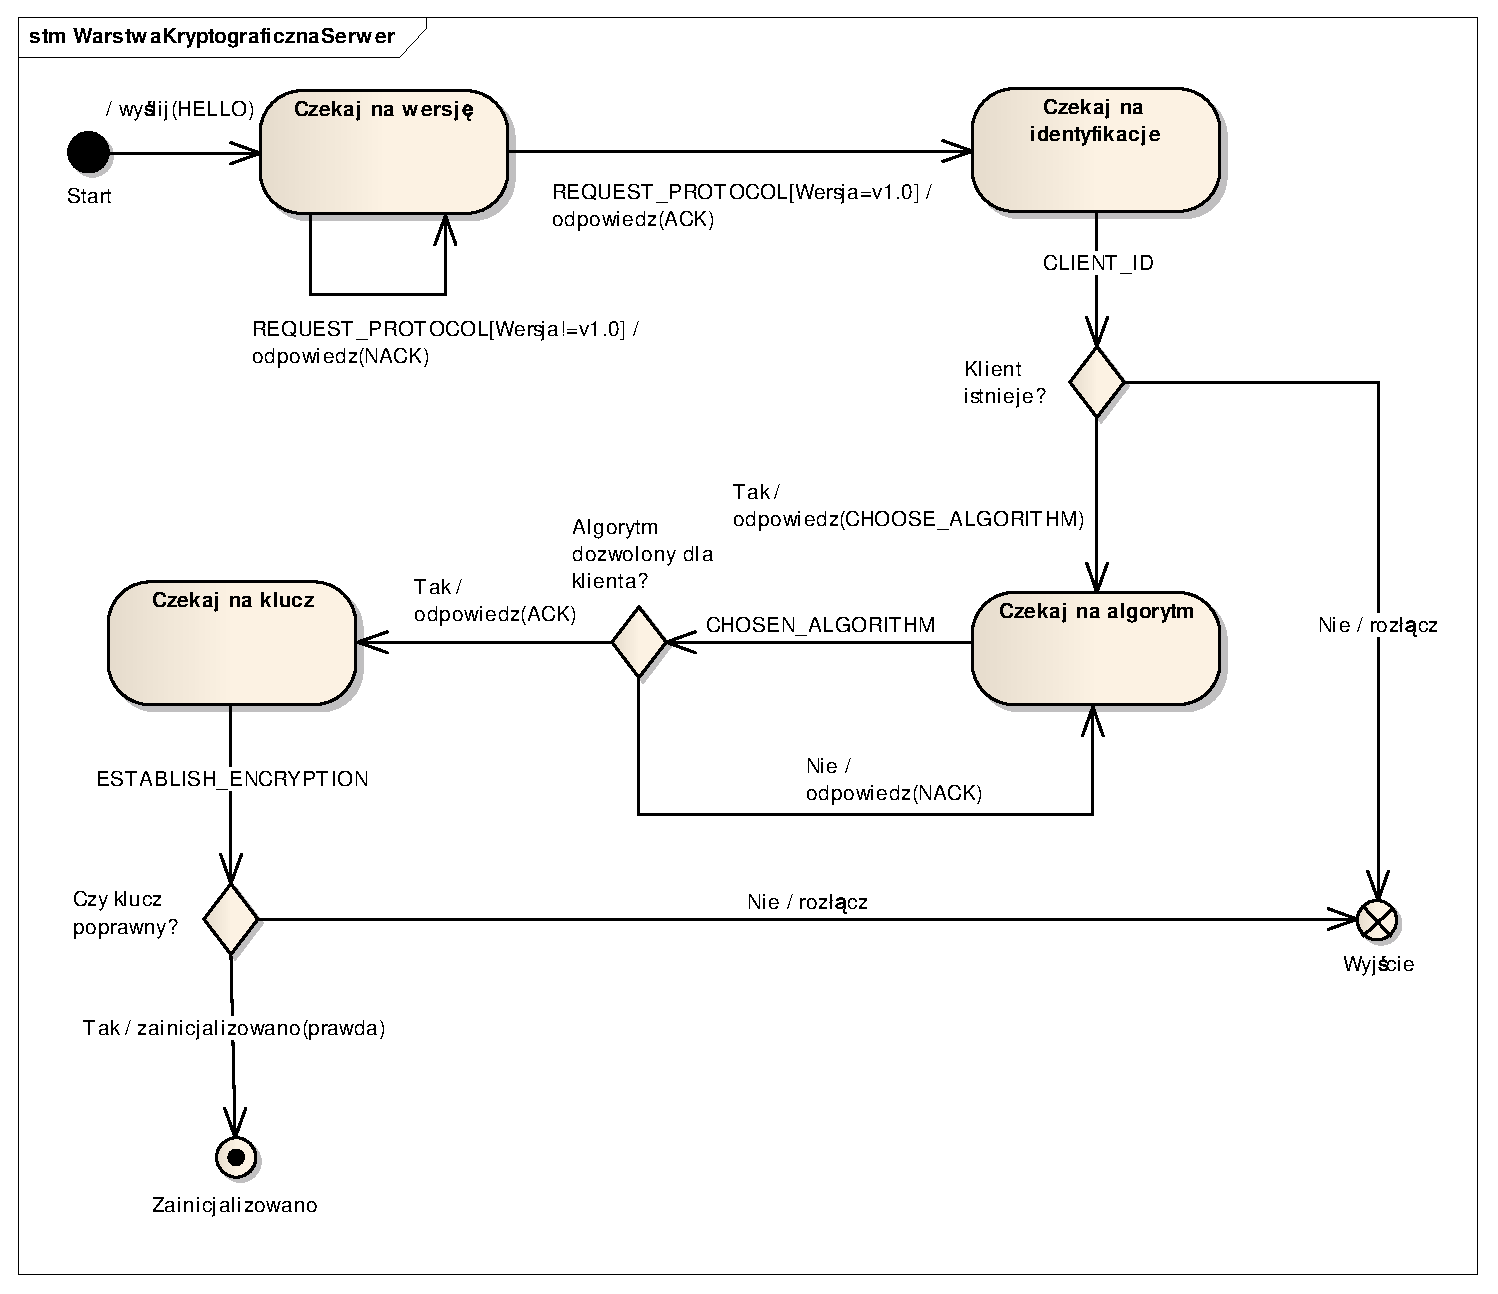
\includegraphics[width=1\textwidth]{img/kryptoSerwer}
\end{figure}

W~zaproponowanej w~tej pracy wersji protokołu kolejnym etapem
inicjalizacji połączenia jest uwierzytelnienie serwera połączone
z~przedstawieniem klienta. Etap ten rozpoczyna się od przesłania przez
klienta jego identyfikatora oraz losowych ośmiu bajtów
danych. Komunikat zaszyfrowany jest kluczem publicznym serwera, zatem
może go odczytać jedynie posiadacz odpowiedniego klucza
prywatnego. Serwer po odebraniu wiadomości odszyfrowuje ją używając
swojego klucza prywatnego. Jeśli wiadomość jest nieczytelna lub klient
o~podanym identyfikatorze nie istnieje serwer niezwłocznie kończy
połączenie. Jeśli wiadomość jest poprawna, a~klient o~podanym
identyfikatorze istnieje serwer wykonuje podpis cyfrowy identyfikatora
oraz losowych bajtów odebranych od klienta. Do klienta odsyłany jest
komunikat zawierający wykonany przez serwer podpis. Klient po
odebraniu podpisu wykonuje weryfikację podpisu na podstawie
wiadomości, która została przesłana do serwera. Jeśli podpis jest
zgodny oznacza to, że urządzenie z którym nastąpiło połączenie jest
posiadaczem odpowiedniego klucza prywatnego, czyli upoważnione przez
administratora do odbierania danych pochodzących od tego klienta.

\begin{figure}[h]
  \caption{Maszyna stanów warstwy kryptograficznej po stronie klienta.}
  \label{fig:kryptoKlient}
  \centering
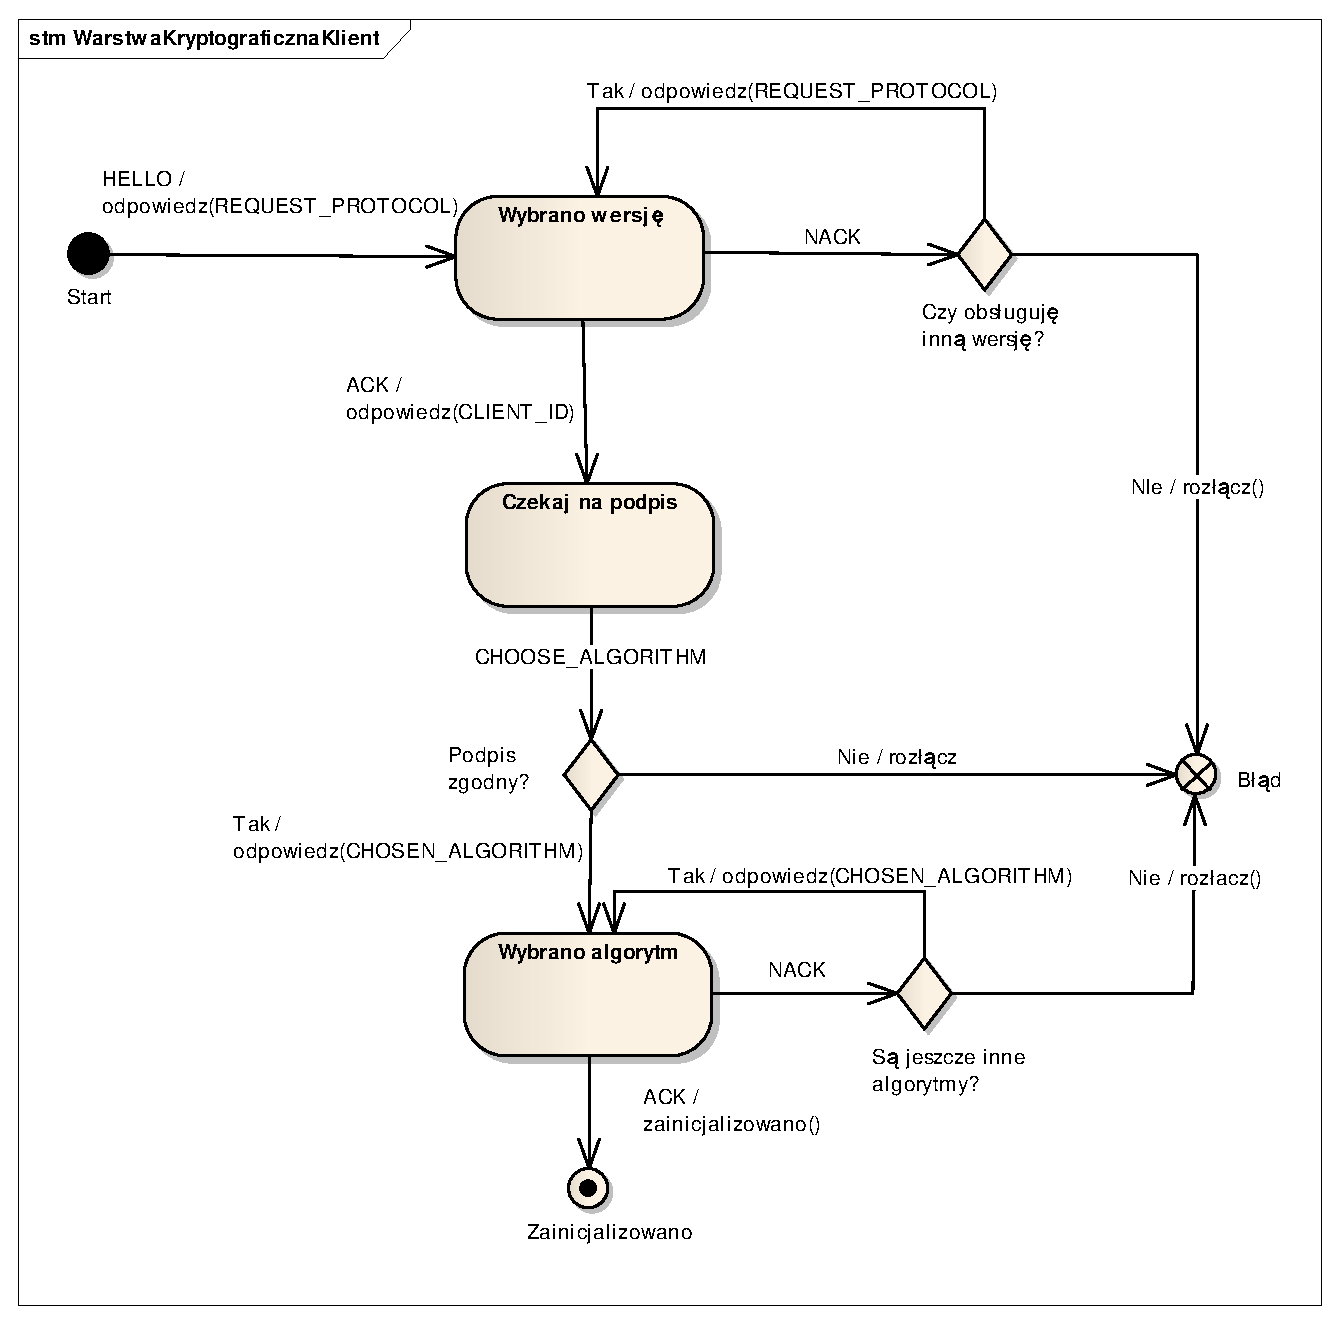
\includegraphics[width=1\textwidth]{img/kryptoKlient}
\end{figure}

\begin{table}[H]
\centering
\caption{Struktura komunikatu identyfikatora klienta }

\begin{tabular}{|p{3cm}|p{3cm}|p{6cm}|}
\hline
Kod CLIENT\_ID & Ciąg losowy & Identyfikator\\
\hline
\end{tabular}
\end{table}

\begin{table}[H]
\centering
\caption{Struktura komunikatu potwierdzającego identyfikator }

\begin{tabular}{|p{6cm}|p{6cm}|}
\hline
Kod CHOOSE\_ALGORITHM & Podpis danych z CLIENT\_ID\\
\hline
\end{tabular}
\end{table}

Ostatnim etapem inicjalizacji komunikacji w~tej warstwie jest
negocjacja algorytmu szyfrowania oraz generacja odpowiedniego klucza
symetrycznego. Klient przesyła do serwera zaszyfrowany kluczem
publicznym komunikat zawierający żądanie algorytmu
symetrycznego. Serwer po odebraniu komunikatu odszyfrowuje go przy
użyciu klucza prywatnego. W zależności od dostępności żądanego
algorytmu, do klienta odsyłany jest komunikat akceptujący lub
odrzucający wybrany algorytm. Klient po odebraniu negatywnego
potwierdzenia może ponownie zażądać innego algorytmu
symetrycznego. Klient po odebraniu komunikatu akceptującego wybrany
algorytm dokonuje generacji klucza symetrycznego, a~następnie oblicza
jego skrót. Tak przygotowany komunikat szyfrowany jest kluczem
publicznym i~przesyłany do serwera. Serwer po odebraniu klucza
sprawdza jego poprawność oraz zgodność z~dołączonym skrótem, co
stanowi ostatni etap inicjalizacji.

\begin{table}[H]
\centering
\caption{Struktura komunikatu żądania algorytmu }

\begin{tabular}{|p{5cm}|p{6cm}|}
\hline
\raggedright{Kod CHOSEN\_ALGORITHM} & Nazwa algorytmu\\
\hline
\end{tabular}
\end{table}

\begin{table}[H]
\centering
\caption{Struktura komunikatu zawierającego klucz symetryczny}

\begin{tabular}{|p{3cm}|p{5cm}|p{3cm}|p{2cm}|}
\hline
Długość skrótu & \raggedright{Kod ESTABLISH\_ENCRYPTION} & \raggedright{Klucz symetryczny} & Skrót \\
\hline
\end{tabular}
\end{table}

Wykonanie inicjalizacji pozwoliło na uzgodnienie w~sposób bezpieczny
klucza symetrycznego. W~dalszej komunikacji wszystkie komunikaty
szyfrowane są z~użyciem wybranego algorytmu symetrycznego. Ponieważ
algorytmy szyfrowania nie zapewniają integralności przesyłanych danych
konieczne jest użycie funkcji skrótu. W~omawianym protokole została
użyta funkcja SHA2. Przygotowanie zatem każdego komunikatu z~danymi
rozpoczyna się od obliczenia skrótu danych. Ponieważ algorytm skrótu
nie był negocjowany konieczne jest dostarczenie długości używanego
skrótu. Długość skrótu wyrażona w bajtach dołączana jest na początku
wiadomości, natomiast sam skrót na końcu. Komunikat przed wysłaniem
szyfrowany jest uzgodnionym kluczem symetrycznym.

\begin{table}[H]
\centering
\caption{Struktura komunikatu danych warstwy kryptograficznej }

\begin{tabular}{|p{3cm}|p{6cm}|p{3cm}|}
\hline
Długość skrótu & Dane & Skrót danych\\
\hline
\end{tabular}
\end{table}

\subsection[Warstwa transportu pomiarów][Warstwa transportu pomiarów]{Warstwa transportu pomiarów}

Warstwa ta zapewnia zapewnia transport wpisów dziennika w~pakietach
o~dowolnym rozmiarze. Wykorzystanie warstw niższych gwarantuje zarówno
poufność jak i~integralność przesyłanych komunikatów. Żadna z~niższych
warstw nie zapewnia jednak uwierzytelnienie klienta, dlatego jest to
również jedno z~zadań tej warstwy.

Inicjalizacja komunikacji w~tej warstwie rozpoczyna się od negocjacji
algorytmu uwierzytelnienia klienta. Serwer przesyła do klienta
komunikat informujący o~konieczności wyboru algorytmu
uwierzytelnienia. Klient przesyła komunikat zawierający nazwę
algorytmu, który ma być użyty do potwierdzenia tożsamości. Serwer po
otrzymaniu komunikatu sprawdza czy żądany algorytm jest dostępny dla
tego klienta. Jeśli nie jest, przesyłany jest komunikat informujący
o~odrzuceniu żądania, a~klient może ponowić żądanie używając innego
algorytmu. Jeśli algorytm wybrany przez klienta jest dostępny
rozpoczyna się proces uwierzytelnienia.

\begin{table}[H]
\centering
\caption{Struktura komunikatu żądania algorytmu uwierzytelnienia }
\begin{tabular}{|p{5cm}|p{6cm}|}
\hline
\raggedright{Kod CHOSEN\_AUTH\_MODULE} & Nazwa algorytmu uwierzytelnienia\\
\hline
\end{tabular}
\end{table}

Uwierzytelnienie klienta wykonywane jest poprzez zewnętrzne moduły,
gdyż protokół komunikacyjny musi być niezależny od protokołu
komunikacyjnego. Algorytm uwierzytelnienia uprawniony jest do
przesyłania dowolnych danych w~obie strony. Jeśli algorytm
uwierzytelnienia odrzuci klienta oznacza to natychmiastowe zamknięcie
połączenia. Pomyślne zakończenie procesu uwierzytelnienia oznacza,
konieczność wykonania sprawdzenia, czy klient posiada zdefiniowane
miejsca do których może przekazywać swoje dane. W przypadku braku
takiego miejsca, aby dane nie zostały utracone do klienta wysyłany
jest komunikat negatywnego potwierdzenia, a~połączenie jest
zamykane. Jeśli co najmniej jedno miejsce docelowe zostało
zdefiniowane do klienta wysyłany jest komunikat informujący
o~oczekiwaniu na przesłanie danych, co kończy proces
inicjalizacji. Przebieg omówionego procesu inicjalizacji oraz
pozostałych elementów protokołu po stronie serwera przedstawia
\ref{fig:transportSerwer}, natomiast po stronie klient
\ref{fig:transportKlient}.


\begin{figure}[ht]
  \caption{Maszyna stanów warstwy transportu pomiarów po stronie serwera.}
  \label{fig:transportSerwer}
  \centering
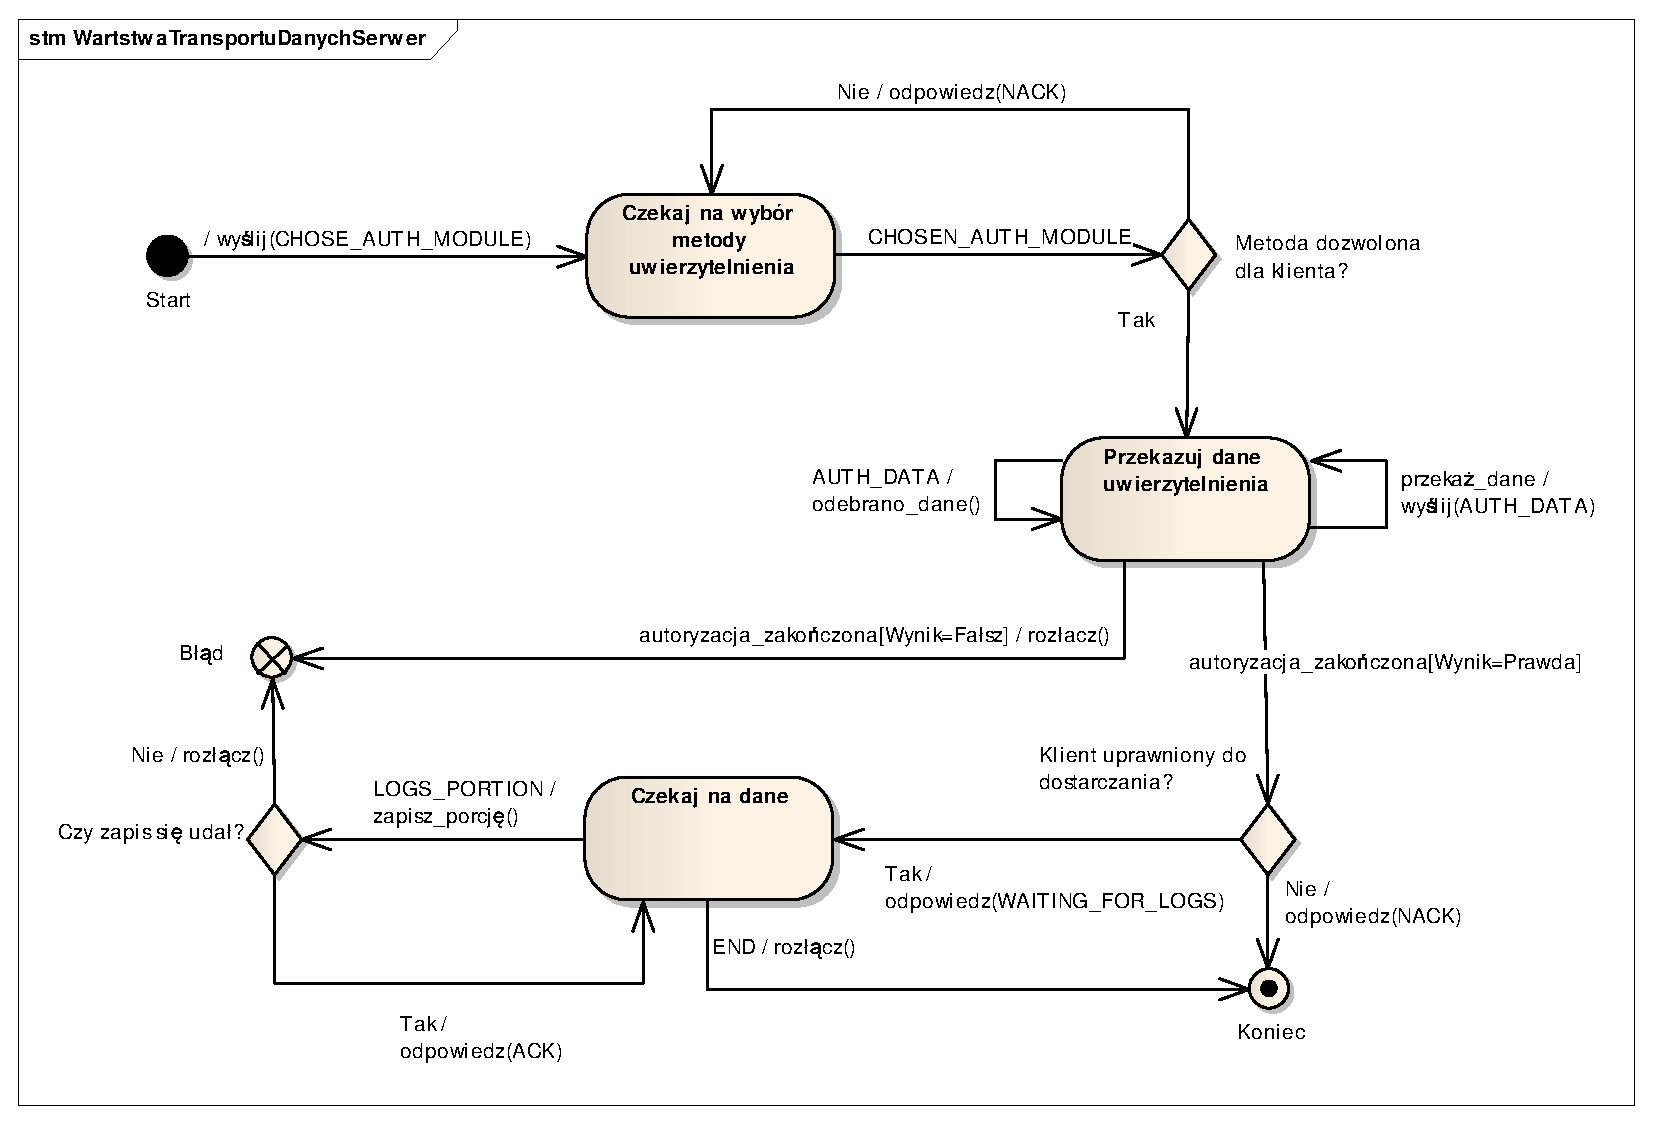
\includegraphics[width=1\textwidth]{img/transpSerwer}
\end{figure}

\begin{figure}[ht]
  \caption{Maszyna stanów warstwy transportu pomiarów po stronie klienta.}
  \label{fig:transportKlient}
  \centering
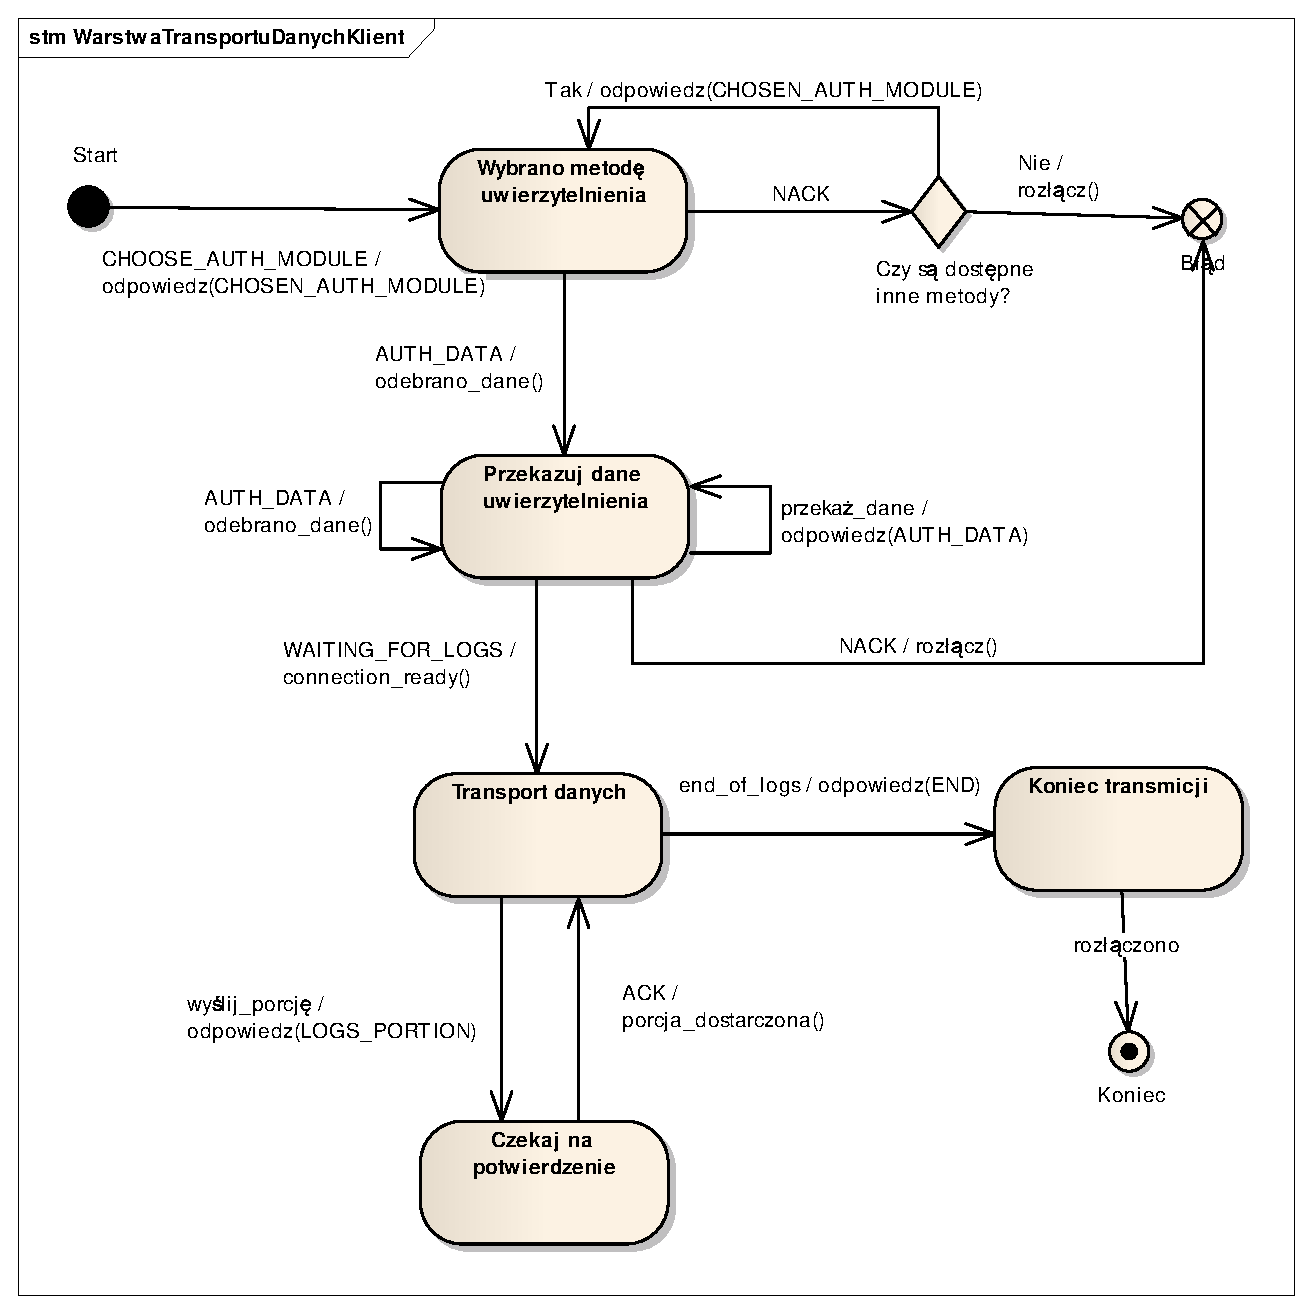
\includegraphics[width=1\textwidth]{img/transpKlient}
\end{figure}

\begin{table}[H]
\centering
\caption{Struktura komunikatu z danymi uwierzytelnienia }
\begin{tabular}{|p{3cm}|p{6cm}|}
\hline
Kod AUTH\_DATA & Dane \\
\hline
\end{tabular}
\end{table}

Dane przesyłane przez klienta znajdują się w pakietach. Po odebraniu
każdego pakietu i~jego pomyślnym przetworzeniu przez aplikację
obliczany jest skrót danych w~nim zawartych. Obliczony skrót jest
następnie przesyłany w~pakiecie potwierdzającym przetworzenie danych.

\begin{table}[H]
\centering
\caption{Struktura komunikatu zawierającego dane }
\begin{tabular}{|p{3cm}|p{6cm}|}
\hline
\raggedright{Kod LOGS\_PORTION} & Dane pomiarów  \\
\hline
\end{tabular}
\end{table}

Pakiet z~danymi może zawierać dowolną liczbę wpisów dziennika. Każdy
wpis powinien posiadać odpowiedni format. W~szczególności każdy wpis
powinien zawierać bajt danych, który pozwala na określenie czy dotyczy
on urządzenia czy usługi. Niezbędne jest również przesłanie stempla
czasu, który determinuje kiedy dany wpis został utworzony. Stempel ten
powinien być zgodny z stemplem czasu systemu Unix oraz być przesłany w
sieciowej kolejności bajtów. Do prawidłowego przekazania wpisu do
systemu monitorującego konieczne jest również dostarczenie nazwy
urządzenia oraz usługi. W~celu umożliwienia oddzielenia tych danych
konieczne jest zakończenie każdego z~tych pól znakiem zerowym. Każdy
wpis powinien również zawierać bajt informujący o~stanie w~jakim jest
dana usługa. Kod ten powinien być zapisany przy użyciu jednego bajtu
w~sposób zgodny z~kodami akceptowanymi przez system monitorujący.

\begin{table}[H]
\centering
\caption{Struktura pojedynczego wpisu dziennika urządzenia }
\begin{tabular}{|p{2cm}|p{3cm}|p{4cm}|p{2cm}|p{2cm}|}
\hline
Kod HOST & Stempel czasu & Nazwa urządzenia & Kod stanu & Wpis  \\
\hline
\end{tabular}
\end{table}

\begin{table}[H]
\centering
\caption{Struktura pojedynczego wpisu dziennika usługi }
\begin{tabular}{|p{2cm}|p{2cm}|p{3cm}|p{2cm}|p{1cm}|p{2cm}|}
  \hline
  \raggedright{Kod SERVICE} & \raggedright{Stempel czasu} & \raggedright{Nazwa urządzenia} & \raggedright{Nazwa usługi} & \raggedright{Kod stanu} & Wpis  \\
  \hline
\end{tabular}
\end{table}

Jeśli odebrane dane posiadają nieprawidłową strukturę, lub klient
dokonał próby przesłania danych, do których przesyłania nie ma
uprawnień połączenie jest natychmiast zamykane. Klient, po przesłaniu
wszystkich danych lub w~chwili zdefiniowanej przez administratora może
zdecydować o~zamknięciu połączenia wysyłając odpowiedni
komunikat. Serwer po odebraniu tego komunikatu zamknie połączenie.


\section[Projekt modułu mobilnego][Projekt modułu mobilnego]{Projekt modułu mobilnego}

Moduł ten jest odpowiedzialny za monitorowanie zadanych parametrów
urządzenia mobilnego. Klienty mobilne są wzajemnie nie zależne i~mogą
operować bez możliwości komunikacji pomiędzy sobą. Konieczne jest
zatem, aby każdy klient mobilny posiadał swoją instancję tego
modułu. W~module tym możemy wyróżnić trzy podstawowe, rozdzielne
funkcjonalnie elementy:

\begin{itemize}
\item element pomiarowy,
\item element komunikacyjny,
\item zestaw wtyczek.
\end{itemize}

Element pomiarowy jest odpowiedzialny za planowanie i~wykonywanie
pomiarów zgodnie z~polityką zdefiniowaną przed administratora. Ponadto
konieczne jest zapewnienie składowania uzyskanych informacji do czasu
udanej synchronizacji z~serwerem. Element komunikacyjny jest to
implementacja opisanego wcześniej protokołu komunikacyjnego dla danej
platformy. Zadaniem tej części jest dostarczenie wyników pomiarów do
miejsc zdefiniowanych przez administratora. Wtyczki są to elementy
bezpośrednio odpowiedzialne za wykonywanie pomiarów zadanych wartości
czy testowanie zdefiniowanych usług. Metoda realizacji wtyczek
uzależniona jest od platformy sprzętowej na jaką przeznaczona jest
dana implementacja modułu. Konieczne jest jednak zapewnienie
niezależności elementu pomiarowego od zestawu wykorzystywanych
wtyczek, aby umożliwić swobodną zmianę zbioru wykorzystywanych
wtyczek.

Implementacja tego modułu musi uwzględniać uwarunkowania sprzętowe jak
i~systemowe platformy na której się znajduje. Urządzenia mobilne są
zazwyczaj zasilane z~własnych akumulatorów dlatego konieczne jest
zastosowanie mechanizmów, które pozwolą na zredukowanie zużycia
energii związanego z~systematycznym wykonywaniem sprawdzeń. Należy
również wspomnieć, iż moduł mobilny odpowiedzialny jest za nadawanie
każdemu z~odczytów stempla czasu uniwersalnego\footnote{Czas
  uniwersalny - średni astronomiczny czas słoneczny na południku
  zerowym.} dokonywanego pomiaru. Na podstawie dokonanej
charakterystyki klienta mobilnego, można poczynić założenie, iż klient
posiada dostęp do punktów synchronizacji czasu. Jest wiele dostępnych
metod synchronizacji czasu na urządzeniu mobilnym, między innymi
pobranie czasu z~sieci GSM czy też z~serwerów czasu światowego, przez
co nie stanowi to dla klienta mobilnego poważnego wymagania.

Klient mobilny po zebraniu porcji wpisów dziennika o~rozmiarze zgodnym
z~polityką administratora, lub po upływie określonego czasu powinien
przesłać posiadane wpisy dziennika do modułu odbiorczego, a~po
uzyskaniu potwierdzenia usunąć je z~urządzenia w~celu oszczędności
pamięci. Możliwa jest również sytuacja, w~której klient mobilny
użytkowany jest przez pewien czas bez dostępu do sieci przez którą
możliwa jest komunikacja z serwerem. W takiej sytuacji moduł mobilny
powinien gromadzić odczyty, aż do czasu uzyskania możliwości
połączenia z~serwerem. Różnorodność platform dostępnych na rynku
sprawia, iż nie można wymagać od modułu odbiorczego dostarczenia
uniwersalnej implementacji protokołu komunikacyjnego. Wymaga się
zatem, aby klient mobilny używał protokołu komunikacyjnego zgodnego
z~protokołem modułu odbiorczego. Konieczne jest również, aby klient
mobilny posiadał możliwość definiowania metod uwierzytelnienia. Należy
również zapewnić możliwość weryfikacji tożsamości serwera, z~którym
nawiązuje się połączenie.

W~ramach systemu monitorowania możliwe jest funkcjonowanie wielu
instancji modułu mobilnego. Instancje te mogą być uruchomione na
bardzo wielu platformach. W~chwili pisania tej pracy nie znaleziono na
rynku żadnej aplikacji przeznaczonej, na platformę mobilną, która
spełniałaby stawiane wymagania. Szczegółowy projekt oraz
implementacja tego modułu dla platformy mobilnej wykracza poza zakres
niniejszej pracy. Podczas okresu testowania wykonanego systemu
wykorzystano moduł mobilny, przeznaczony dla platformy Android. Został
on zaprojektowany i~zaimplementowany przez Pana Marcina
Kubika. Szczegółowy opis tej implementacji klienta mobilnego można
znaleźć w~\cite{book:pracaKubika}.

\section[Projekt modułu odbiorczego][Projekt modułu odbiorczego]{Projekt modułu odbiorczego}
\label{sec:ProjModOdb}

Moduł ten pośredniczy w~przekazywaniu danych pomiędzy modułem mobilnym
a~modułem podstawowym. Uruchomiony jest on na serwerze, który posiada
dostęp do zarówno do sieci wewnętrznej instytucji, jak i~do sieci,
w~której funkcjonują klienty mobilne, w~szczególności do sieci
Internet. Możliwe jest również umieszczenie tego modułu na tym samym
urządzeniu, co rdzeń monitorujący odpowiedzialny z~przetwarzanie
danych pochodzących od klientów mobilnych.

Moduł ten składa się z jednego programu, którego zadaniem jest
przekazywanie danych od klientów mobilnych zgodnie ze zdefiniowaną
polityką. Znaczna część logiki programu oraz polityka dostarczania
danych jest konfigurowana przy pomocy pliku konfiguracyjnego, co
umożliwia jej zmianę bez konieczności ponownej kompilacji
programu. Plik ten zawiera również definicję klientów, którzy są
uprawnieni do przekazywania danych. Każdy klient może posiadać wiele
urządzeń, a każde z~urządzeń wiele usług. Zgodnie z~protokołem
komunikacyjnym przed przesłaniem danych występuje etap
uwierzytelnienia klienta. Przekazywanie danych możliwe jest jedynie po
zakończeniu pozytywnym potwierdzeniu tożsamości
klienta. Wysokopoziomowy model logiczny omawianego programu składa się
zatem z~następujących elementów:

\begin{itemize}
\item dostawca danych,
\item kanał komunikacyjny,
\item konsument danych.
\end{itemize}

Dostawca danych jest to fragment programu odpowiedzialny za odebranie
oraz kontrolę danych pochodzących od klienta. Zawiera on więc
implementację protokołu komunikacyjnego oraz wykorzystuje dostępne
w~programie algorytmy kryptografii oraz uwierzytelnienia zgodnie
z~konfiguracją. W celu umożliwienia współpracy różnych protokołów
komunikacyjnych możliwe jest używanie jednocześnie wielu dostawców
danych. Kanał komunikacyjny stanowi natomiast niezawodne
asynchroniczne medium komunikacyjne pomiędzy dostawcą, a
konsumentami. Dostawca danych zobowiązany jest do dostarczenia danych
jedynie do jednego miejsca, czyli kanału komunikacyjnego. Logika
zawarta w~kanale wyznacza natomiast na podstawie zdefiniowanej
polityki podzbiór konsumentów danych, którzy powinni powinien otrzymać
przekazane danych. Możliwe jest definiowanie polityki dostarczania
danych zarówno na podstawie informacji o~kliencie od którego pochodzą
dane, jak i~na podstawie informacji o~dostawcy który odebrał
dane. W~celu przyśpieszenia komunikacji z~klientem mobilnym
potwierdzenie przetworzenia danych zawarte w~protokole komunikacyjnym
wysyłane jest niezwłocznie po przekazaniu danych do kanału
komunikacyjnego. Konieczne jest zatem zapewnienie niezawodności kanału
komunikacyjnego, aby możliwe było gwarantowanie, że dane, które do
niego zostały przekazane będą dostarczone do wskazanych
odbiorców. Odbiorca danych jest to element programu odpowiedzialny za
odpowiednie formowanie danych oraz przekazanie ich do modułu
podstawowego. Dzięki możliwości dostarczania danych do wielu
odbiorców, możliwe jest nie tylko przekazywanie danych do systemu
monitorującego lecz również wykonywanie np. kopi zapasowej otrzymanych
danych. Przykłądowy schemat logiczny dla dwóch dostawców danych oraz
trzech konsumentów został przedstawiony na \ref{fig:odbiorczy}

\begin{figure}[ht]
  \caption{Diagram architektury modułu odbiorczego}
  \label{fig:odbiorczy}
  \centering
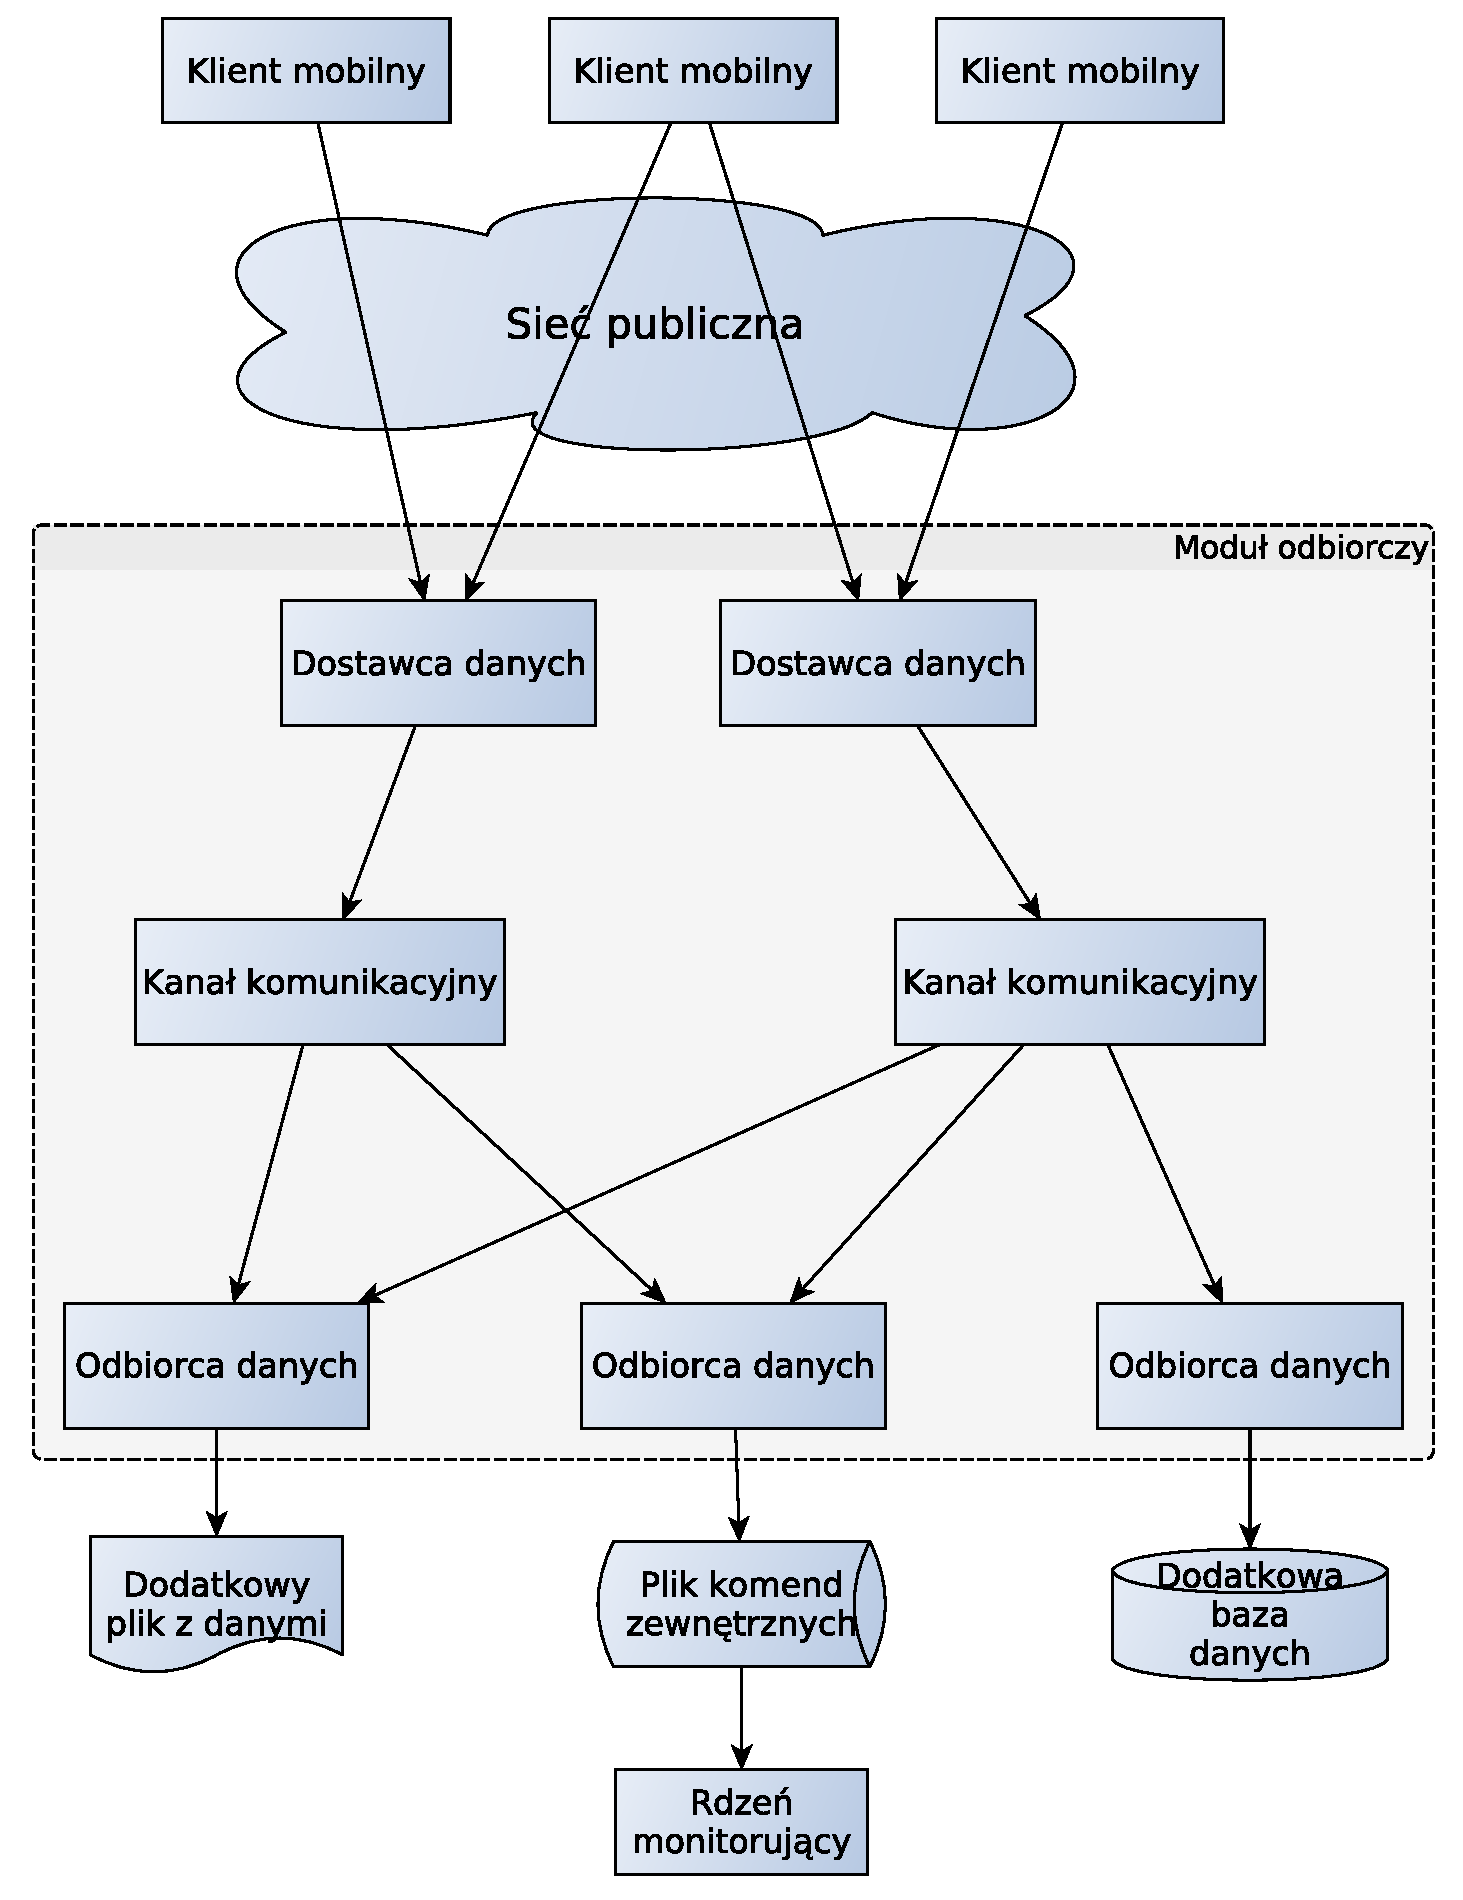
\includegraphics[width=0.7\textwidth]{img/odbiorczy}
\end{figure}

Wymagania przedstawione w~\ref{chap:Wymagania} wymuszają umożliwienie
dodawania nowych algorytmów zarówno kryptograficznych jak i~algorytmów
uwierzytelnienie klienta. W~celu spełnienia tych wymagań wyróżnione
zostały w!programie również dwa moduły pomocnicze:

\begin{itemize}
\item moduł uwierzytelnienia,
\item moduł kryptograficzny.
\end{itemize}

Moduł uwierzytelnienia stanowi bibliotekę algorytmów uwierzytelnienia
klienta, które mogą być wykorzystane przez dostawców danych w~celu
weryfikacji tożsamości klienta. Moduł kryptograficzny stanowi
natomiast bibliotekę algorytmów kryptografii symetrycznej,
asymetrycznej oraz funkcji skrótu. Umożliwia to realizację procesu
negocjacji algorytmu symetrycznego wykorzystywanego przez protokół
komunikacyjny. Ponieważ różnice pomiędzy poszczególnymi protokołami
komunikacyjnymi mogą być niewielkie w~programie wyodrębniono również
moduł implementujący poszczególne warstwy protokołu. Umożliwi to w
przyszłości szybką modyfikację protokołu komunikacyjnego lub dodanie
nowego.

